\chapter{Grundlagen der Implementierung} % (fold)
\label{cha:implementierung_Überblick}

Wie im Kapitel "Design" gefordert, wurde zur Umsetzung des Werkzeugs ein "Tangible Tabletop Interface" verwendet. Tabletop Interface zeichnen sich im Generellen dadurch aus, dass im Gegensatz zu handelsüblichen Rechnern nicht nur die Software sondern auch die Hardware applikationsspezifisch ist und nicht generisch eingesetzt werden kann. Die Hardware bildet dabei einen Teil oder die gesamte Benutzungsschnittstelle ab. Im speziellen Fall eines "Tangible Tabletop Interfaces" basiert der Benutzerinteraktion auf der Verwendung physischer Bausteine ("Tokens"), die auf der physischen Oberfläche des Interfaces manipuliert werden. Dieses Paradigma wird ergänzt von Tabletop Interfaces, die die Benutzerinteraktion ausschließlich auf Gesten bzw. Berührungen der Oberfläche abbilden (horizontal verbaute "Touch-" bzw. "Multi-Touch-Displays").

REFs!!! Die Entwicklung von Tabletop Interfaces begann Mitte der 1990er-Jahren mit den Arbeiten von Ishii \& Ullmer. Auch die erste Anwendung, die sich mit Modellierungs-Ansätzen mit Hilfe von Tabletop Interfaces konzentriert, stammt aus dieser Zeit. Mit dem fortschreiten der technologischen Entwicklung ist heute ein Status erreicht, in dem mit Hilfe generischer Identifikations-Frameworks schnell und ohne großen Aufwand Applikationen mit "tangiblen" Inputkanälen erstellt werden können. Zur Zeit noch im Prototypenstatus befinden sich Ansätze, die sich mit generischen Möglichkeiten des tangiblen Informationsoutputs beschäftigt. Der Rückkanal vom Rechner zum Benutzer wird heute zumeist mit der Projektion von Inhalten auf die Arbeitsoberfläche umgesetzt.

In den folgenden Abschnitten wird die historische Entwicklung von Tabletop Interfaces sowie der aktuelle Stand der Entwicklung im Anwendungsbereich dieser Arbeit betrachtet. Es werden dabei die grundlegenden Konzepte und Eigenschaften der jeweiligen Arbeiten betrachtet und das Potential hinsichtlich der Umsetzung von in Kapitel XY identifizierten Anforderungen an das hier entwickelte Werkzeug betrachtet. 

\section{Historische Entwicklung von Tangible Interfaces} % (fold)
\label{sec:entwicklung_tangible_interfaces}

Der Begriff der Tangible bzw. Graspable Interfaces – also der "berührbaren" oder "begreifbaren" Benutzungsschnittstellen — stammt aus der Mitte der neunziger Jahre des zwanzigsten Jahrhunderts. \citet{Fitzmaurice95} werden im Allgemeinen als die ersten betrachtet, die den Begriff des "Graspable User Interfaces" prägen und damit die Manipulierbarkeit digitaler Information durch physische Mittel beschreiben. \citet{Fitzmaurice96} präzisiert später den Begriff durch die Abgrenzung zwischen (herkömmlichen, maus-, tastatur- und bildschirmbasierenden) zeitlich gemultiplexten Schnittstellen, bei denen der Informationsaustausch zwischen Benutzer und System über einen Kanal zeitlich hintereinander erfolgt und den (neuartigen, berührbaren) räumlich gemultiplexten Schnittstellen, bei denen mehrere Kanäle gleichzeitig zur Interaktion zwischen Benutzer und System verwendet werden können. 

Der Begriff des "Tangible User Interfaces" wurde kurz danach bzw. parallel dazu von \citet{Ishii97} eingeführt. \citeauthor{Ishii97} verfolgen dabei bei der Definition den umgekehrten Weg und sprechen von einer "Augmentation der realen Welt durch eine Kopplung von digitaler Information and physische Objekte"\footnote{\emph{“augment the real physical world by coupling digital information to everyday physical objects and environments”}\citep{Ishii97}}. 

\subsection{Ubiquitous Computing}

\subsection{Augmented Reality} 

% subsection tangibles_historischer_hintergrund (end)

\section{Konzeptualisierung und Klassifikation von Tangible Interfaces} % (fold)
\label{sec:konzeptualisierungen_von_tangible_interfaces}

Die Entwicklung des Forschungsgebiets der "Tangible Interfaces" wurde von mehreren konzeptuellen Arbeiten maßgeblich beeinflusst. Die dort vorgeschlagenen Erklärungsmodelle definieren das Gebiet und grenzen es gegenüber anderen Forschungsbereichen ab. Sie dienen außerdem als Grundlage für Erklärung und Konzeption konkreter Tangible Interfaces. Im Folgenden wird die historische Entwicklung dieser konzeptuellen Modelle beschrieben und auf deren Spezifika eingegangen.

Zur strukturierten Betrachtung von Tangible Interfaces ist es außerdem notwendig, jene Dimensionen zu identifizieren, an denen sich einzelne Tangible Interfaces einordnen und unterscheiden lassen. Die Ausprägungen dieser Dimensionen liefern kombiniert ein Begriffssystem, dass bei der Aufbereitung von unterschiedlichen Ansätzen im Bereich der Tangible Interface sowie deren Vergleich helfen kann. Die hier vorgestellten Ansätze tragen unterschiedlich detailliert und aus unterschiedlichen Gesichtspunkten zu dieser Thematik bei. Die einzelnen Ansätze werden hier dargestellt und in Kapitel XY auf das in dieser Arbeit entwickelte System angewandt um so das System-Design aus konzeptueller Sicht zu reflektieren und potentielle Verbesserungs- und Erweiterungsmöglichkeiten zu identifizieren.

Allgemein ist anzumerken, dass eine Vielzahl von Ausdrücken im sich entwickelnden Forschungsgebiet mehrfach belegt wurden und/oder nicht eindeutig definiert sind. Im Folgenden werden die Ausdrücke der jeweiligen Autoren übernommen, eine Interpretation bzw. Abbildung auf die Terminologie anderer Autoren wird nur vorgenommen, wo sie im jeweiligen Artikel explizit angeführt wurde. In der Zusammenfassung dieses Abschnitts wird versucht, die unterschiedlichen Terminologien nochmals zusammenzufassen und einen Satz an Ausdrücken festzulegen, der im Folgenden für diese Arbeit Anwendung findet.

Am Ende jeder Beschreibung sind in einer tabellarischen Zusammenfassung jeweils die zentralen Konzepte und Beiträge des Ansatzes angeführt. Die Tabelle weist einheitlich Einträge zu folgenden Themen auf:
\begin{description}
 \item[Kategorien] Kategorien von Tangible Interfaces, die im Beitrag identifiziert werden  (inkl. Unterscheidungsmerkmal zur Kategoriebildung)
 \item[Konzepte] Konzepte, die bei der Betrachtung bzw. beim Design eines Tangible User Interfaces zur Anwendung kommen 
 \item[Eigenschaften] Eigenschaften, die ein Tangible User Interface bzw. dessen Komponenten aufweisen können
 \item[PD-Brücke] Aussagen, die der Beitrag zur Natur oder Ausgestaltung der Brücke zwischen physische und digitaler Welt macht
\end{description}

Wird in einem Beitrag keine Aussage zu einem oder mehreren dieser Themen gemacht, so ist dies expizit durch "---" angeführt.

-- evtl. Kurzüberblick (definition list) über die Ansätze, die jetzt kommen --


\subsection{Graspable User Interfaces}

\citeauthor{Fitzmaurice96} legt in jener Arbeit, in der es den Begriff des "Graspable User Inferfaces" prägt \citep{Fitzmaurice96}, auch Eigenschaften fest, anhand deren sich die "Graspability" einer Benutzungsschnittstelle zeigt und beurteilen lässt. Diese Beurteilung erfolgt auf einer generischen Skala mit Ausprägungen von "niedrig" bis "hoch", wobei "hohe" Werte in mehreren Eigenschaften auf eher hohe "Graspability" hinweist.

\subsubsection{Space Mulitplexing}
\subsubsection{Concurrency}
\subsubsection{Physical Form}
\subsubsection{Spartially aware}
\subsubsection{Spatial recofigurability}

\begin{tabular}{| p{3cm} | p{10cm} |}
  \hline
  Kategorien & --- \\ \hline
  Konzepte & --- \\ \hline
  Eigenschaften & --- \\ \hline
  PD-Brücke & --- \\ \hline
\end{tabular} 

\subsection{Bricks} % (fold)
\label{sub:bricks}

\begin{tabular}{| p{3cm} | p{10cm} |}
  \hline
  Kategorien & --- \\ \hline
  Konzepte & --- \\ \hline
  Eigenschaften & --- \\ \hline
  PD-Brücke & --- \\ \hline
\end{tabular} 

% subsection bricks (end)

\subsection{Tangible Bits}
\label{sub:tangible_bits}

\citet{Ishii97} stellen in ihrer Arbeit den Ansatz der „Tangible Bits“ vor, der die virtuelle Welt mit der realen Umwelt verknüpfen soll. Dabei wird digitale Information mit realen Objekten oder Phänomenen gekoppelt und so „tangibel“. Die Autoren unterscheiden drei grundsätzliche Kernkonzepte, die den Ansatz umsetzen:
\begin{description}
	\item[Interactive Surfaces], bei denen beliebige Oberflächen in der realen Welt (etwa Wände oder Schreibtische) zu aktiven Schnittstellen zur virtuellen Welt werden,
	\item[Coupling Bits and Atoms], wo physische Objekte mit ihnen zuzuordnender Information gekoppelt werden, so das die realen Objekte zu Trägern von und Schnittstellen zu digitaler Information werden und
	\item[Ambient Media], bei deren Einsatz über die Umgebung der Benutzer Information vermittelt wird (z.B. mittels Veränderung der Beleuchtung), ohne die eigentliche Tätigkeit zu unterbrechen. 
\end{description}

Die Autoren ordnen Tangible Bits an die Schnittstelle zwischen den Forschungsgebieten „Ubiquitous Computing“ und „Augmented Reality“ ein. „Ubiquitous Computing“ \citep{Weiser91} beschäftigt sich mit Anwendungen, in denen Computer nicht mehr als als solche wahrnehmbare Geräte eingesetzt werden, sondern in der Umgebung integriert sind und von Benutzern nicht mehr bewusst wahrgenommen sondern nur noch als Teil der Alltagswelt benutzt werden. Tangible Bits erben von dieser Forschungsrichtung die Idee der physischen, natürlichen Interaktion zwischen Benutzern und Rechner, unterscheiden sich aber insofern, als das nach wie vor ein Interface zur virtuellen Welt vorhanden ist, diese also zum Teil noch bewusst wahrgenommen wird. In diesem Aspekt ähneln Tangible Bits den Ideen die aus der „Augmented Reality“ Forschung stammen. Augmented Reality beschäftigt sich mit Methoden, die die reale Welt mit digitaler Information nahtlos ergänzen bzw. anreichern. Vor allem im Bereich der Ausgabetechnologien werden bei Tangible Bits viele aus dem „Augmented Reality“-Bereich stammende Konzepte eingesetzt.

Nach der Einordnung stellen die Autoren Prototypen vor, die das Konzept der „Interactive Surfaces“ als auch der „Ambient Media“ umsetzten. Erwähnenswert ist im Zusammenhang mit dieser Arbeit der Prototyp „metaDESK“ \citep{Ullmer97}, eine interaktive Oberfläche in Form eines Tisches, auf der die klassischen Interaktionselemente eines \gls{GUI} in die reale Welt transferiert wurden. Dabei wurden die \gls{GUI}-Elemente auf \gls{TUI}-Elemente abgebildet\footnote{dies stellt im Übrigen die historisch erste Erwähnung des Begriffs „Tangible User Interface“ dar}: 
\begin{itemize}
	\item Windows werden auf „Lenses“ abgebildet, also Linsen, die Information zu realen, physischen Elementen anzeigen.
	\item Icons werden in der physischen Welt als „Phicons“ abgebildet und sind im wesentlichen phyischen Objekte, die Information repräsentieren.
	\item Menüs werden durch „Trays“ repräsentiert, in denen Phicons an unterschiedlichen Stellen abgelegt werden können, wobei die Ablageposition jeweils an eine spezifische Operation gebunden ist. 
	\item Handles (Elemente zur Manipulation von GUI-Objekten) werden durch „Phandles“ abgebildet, die im Wesentlichen Phicons sind, die zur Eigabe von Information verwendet werden können.
	\item Widgets (Kontroll- und Steuerelemente) werden durch „Instruments“ abgebildet, welche Phicons sind, die zur Steuerung der jeweiligen Applikation dienen.
\end{itemize}

Ohne hier weiter auf die Beispiele der Autoren einzugehen, ist doch das den Prototypen zugrunde liegende Designkonzept erwähnenswert, etablierte Metaphern aus der realen oder digitalen Welt für die Benutzerinteraktion zu verwenden. In der Diskussion ihrer Ergebnisse identifizieren die Autoren die Thematik der Metaphern, die die Brücke zwischen realer und virtueller Welt schlagen, als eine der interessantesten offenen Fragen für weitere Forschung auf dem Gebiet. Als Schlussfolgerung ihrer Erfahrungen mit den erstellten Prototypen schlagen sich außerdem vor, „optischen“ Metaphern besondere Aufmerksamkeit zu schenken, da diese für den Brückenschlag besonders geeignet wären. 

Als optische Metaphern verwenden die Autoren vor allem Beleuchtung, Schattenwurf und Linsen. Sie bilden diese realen Phänomene auf die Schnittstelle zwischen digitaler und realer Welt ab, so dass z.B. digitale Beleuchtung Information sichtbar macht, die in „unbeleuchteten“ Gebieten fehlt, dass reale Objekte digitale Schatten werfen können und so zusätzliche Information transportieren oder dass eine digitale Linse verwendet wird, um reale Objekt „näher“ zu betrachten und Zusatzinformation einzublenden. Bei der Verwendung von Methaphern wird darauf hingewiesen, das es wichtig sei, auf ein realitätsgetreues Verhalten der digital augmentierten Artefakte zu achten, um eine nahtlose Integration der digitalen Information in die reale Welt zu ermöglichen.

\begin{tabular}{| p{3cm} | p{10cm} |}
  \hline
  Kategorien & Interactive Surfaces, Coupling Bits and Atoms, Ambient Media (Einordnung nach Anwendungsfall) \\ \hline
  Konzepte & Lenses, Phicons, Tray, Phandles, Instruments \\ \hline
  Eigenschaften & --- \\ \hline
  PD-Brücke & zentraler Aspekt: Verwendung etablierter Metaphern \\ \hline
\end{tabular} 

\subsection{Containers, Tokens und Tools}
\label{sub:containers_tokens_tools}

\citet{Holmquist99} legen ihre Arbeit als konzeptuelle Betrachtung von interaktiven Systemen an, in denen physische Objekte verwendet werden, um auf digitale Information zuzugreifen bzw. diese zu manipulieren. Das Einteilungsschema, das die Autoren vorschlagen, basiert auf der Art und Weise, in der Information an diese physischen Objekte gebunden ist. Grundsätzlich unterschieden sie zwischen \emph{Containern}, \emph{Tokens} und \emph{Tools}, wobei eine exakte Abgrenzung bzw. eindeutige Zuordnung zu einer Kategorie nicht immer möglich und sinnvoll ist.

Der hier vorgestellte Ansatz fokussiert auf die physische Interaktion als Eingabemedium, auf den Aspekt der Informationsausgabe wird nicht eingegangen. Dies ist für das Verständnis der folgenden Beschreibungen im Kontext der späteren historischen Entwicklung wichtig und muss bei der Anwendung dieses Ansatzes berücksichtigt werden. 

\subsubsection{Containers}

Als Container werden alle jene Objekte bezeichnet, an die beliebige digitale Information gebunden werden kann. Eine Container ist also ein unspezifisches physisches Objekt in einem Tangible User Interface. Sein Aussehen oder andere physische Eigenschaften lasst keine Aussage über die Art der angebundenen Information bzw. die Information selbst zu. 

Beliebige physische Objekte können als Container agieren, sofern sie die Möglichkeit bieten, Information in bzw. auf ihnen abzulegen oder von einer Infrastruktur eindeutig identifizierbar sind, so dass Information über die eindeutige Identifikation an sie gebunden werden kann. Container agieren somit ausschließlich als physische Informationsträger und können als solche verwendet werden, um Information zwischen Systemen zu transportieren. 

Ein typisches Beispiel ist die Verwendung eines Füllfederhalters als Container, an den beliebige Information gebunden werden kann, um diese von einem Ort zum anderen transportieren zu können. Der Füllfederhalter steht in keinem direkten Zusammenhang mit der angebundenen Information, aus seinem Erscheinungsbild oder seinen Eigenschaften kann nicht auf die angebundene Information geschlossen werden.

\subsubsection{Tokens}

Tokens sind physische Objekte, deren äußeres Erscheinungsbild bzw. deren Eigenschaften in irgendeiner Weise mit der durch sie repräsentierten Information zusammenhängen. Das physische Objekte und die angebundene Information sind nicht mehr voneinander unabhängig sondern stehen in eine konzeptuellen Zusammenhang. Die äußere Form oder andere physische Eigenschaften dienen of als Hinweis auf die angebundenen Informationsart oder stehen sogar in Zusammenhang mit der konkrekt angebundenen Information.

Ein typisches Beispiel für ein Token wäre ein Buch, an das über eine eindeutige Identifikation (etwa ein \gls{RFID}-Tag) der jeweilige Text oder Zusatzmaterial gebunden wird. Das physische Buch steht dabei in dirketem Zusammenhang mit der angebundenen digitalen Information.

\subsubsection{Tools}
Tools sind physische Elemente, die nicht Information, sondern Funktionen repräsentieren. Die Anwendung von Tools hat dabei nicht unbedingt physische Auswirkungen, jene digitalen, virtuellen Objekte, auf die das Tool angewandt wird, werden aber entsprechend der Funktion des Tools manipuliert.

Beispiele für Tools sind physische Objekte, die zur Auswahl digitaler Objekte dienen oder Objekte wie Linsen, deren Anwendung zusätzliche Information zu anderen Containern oder Tokens abruft.

\subsubsection{Zugriff auf und Interaktion mit Tokens und Containern}

Der Zugriff auf die Information, die an ein Token oder einen Container gebunden ist, erfolgt über \emph{Information Faucets} (also "Informations-Zapfhähne" oder "-Armaturen"). Diese Faucets sind aktive Komponenten (im Gegensatz zu Tokens und Containern, die im Allgemeinen passive Komponenten sind, also keine dedizierte Elektronik enthalten), deren Aufgabe darin besteht, aus Tokens oder Containern, die in deren Reichweite gelangen, die angebundene Information zu extrahieren und auszugeben. Faucets können auch dazu verwendet werden, den Zugriff auf Information einzuschränken. So kann die Ausgabe von Information an eine bestimmte Kombination von Tokens oder Containern gebunden werden oder von einem bestimmten Aufenthaltsort abhängig gemacht werden.

Die Anbindung von Information an ein Token oder einen Container kann ebenfalls eingeschränkt sein, bzw. ist im Fall von Tokens per Definition durch den notwendigen Zusammenhang zwischen physischem Element und Information eingeschränkt. Neben dieser konzeptuell notwendigen Einschränkung können auch weitere Regeln geprüft werden oder z.B. die Bindung zwischen Objekt und Information statisch (d.h. unveränderbar) gespeichert werden. 

\begin{tabular}{| p{3cm} | p{10cm} |}
  \hline
  Kategorien & --- \\ \hline
  Konzepte & Container, Token, Tool, Faucet \\ \hline
  Eigenschaften & --- \\ \hline
  PD-Brücke & Zugriff auf an physische Elemente gebundene Information nur via Faucets, kein direkter Zugriff vorgesehen \\ \hline
\end{tabular} 

\subsection{Embodied User Interfaces} % (fold)
\label{sub:embodied_user_interfaces}

\citep{Fishkin98}\citep{Fishkin00}

\begin{tabular}{| p{3cm} | p{10cm} |}
  \hline
  Kategorien & --- \\ \hline
  Konzepte & --- \\ \hline
  Eigenschaften & --- \\ \hline
  PD-Brücke & --- \\ \hline
\end{tabular} 

% subsection embodied_user_interfaces (end)

\subsection{Tangible Objects Meaning}
\citep{Underkoffler99}

\begin{tabular}{| p{3cm} | p{10cm} |}
  \hline
  Kategorien & --- \\ \hline
  Konzepte & --- \\ \hline
  Eigenschaften & --- \\ \hline
  PD-Brücke & --- \\ \hline
\end{tabular} 

\subsection{Das MCRpd Interaktions-Modell}
\label{sub:mcrpd}

Basierend auf früheren Arbeiten entwickeln \citet{Ullmer00} ein Interaktionsmodell zur Beschreibung von Tangible User Interfaces. Es handelt sich bei dieser Arbeit um den ersten Ansatz, der sich der Domäne aus Sicht der Systemstruktur nähert und nicht ausschließlich eine reine Klassifikation nach bestimmten Merkmalen eines Systems vornimmt.

Die Autoren grenzen \glspl{TUI} von \glspl{GUI} insofern ab, als das \glspl{TUI} über eine nahtlose Integration zwischen Repräsentation des Systemzustandes und dessen Kontrolle aufweisen (im Gegensatz zu \glspl{GUI}, bei denen der Systemzustand über einen graphischen Kanal ausgegeben wird und über andere Kanäle, etwa Tastatur und Maus, kontrolliert wird). Mit der Forderung nach nahtloser Integration von Repräsentation und Kontrolle -- also im Wesentlich einer Einheit von Eingabe- und Ausgabe-Kanälen -- wird ein eher striktes, eingeschränktes Verständnis von \glspl{TUI} propagiert. Als Tangible User Interface kann ein System demnach nur bezeichnet werden, wenn es Ein- und Ausgabe kohärent über einen Kanal führt.


\begin{figure}[htbp]
	\centering
		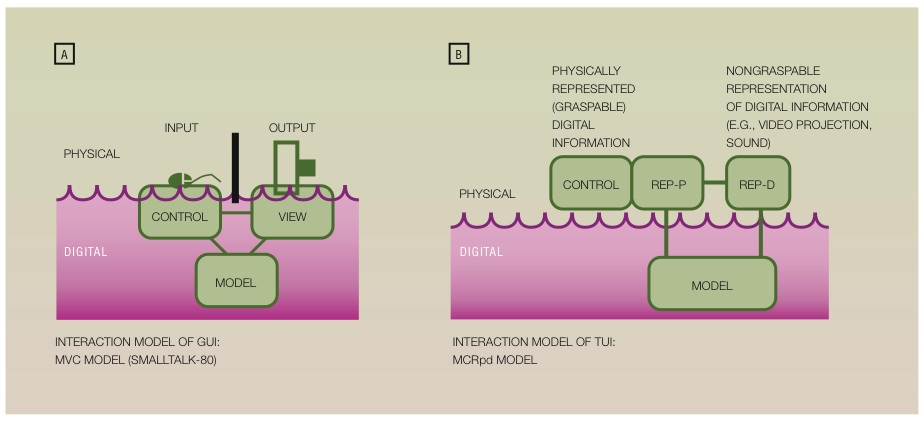
\includegraphics[width=12cm]{img/ImplementierungUeberblick/MCRpd.jpg}
	\caption[Interaktionsmodelle für GUI und TUI]{Interaktionsmodelle für GUI und TUI (übernommen von \citet{Ullmer00})}
	\label{fig:img_ImplementierungUeberblick_MCRpd}
\end{figure}

Diese Sichtweise setzten die Autoren in der Folge in einem Interaktionsmodell für \glspl{TUI} um, dass die Struktur eines Tangible User Interfaces konzeptuell beschreibt. Das Modell wird dabei analog zum \gls{MVC}-Modell konzipiert, das für \glspl{GUI} zum Einsatz kommt und entsprechend der engeren Kopplung zwischen Repräsentation und Kontrolle als \gls{MCRpd}-Modell bezeichnet (siehe Abbildung \ref{fig:img_ImplementierungUeberblick_MCRpd}). An der Gegenüberstellung zwischen \gls{MVC}- und \gls{MCRpd}-Modell wird die Unterscheidung zwischen \gls{GUI} und \gls{TUI} deutlich. Beiden Ansätzen ist gemein, dass der Systemzustand im Rechner durch ein \emph{Model} dargestellt wird. Unterschiede zeigen sich in der Art der Manipulation und Manifestation dieses \emph{Models}. Bei \glspl{GUI} ist Eingabe und Ausgabe strikt getrennt. Die Manipulation des Systemzustandes erfolgt durch die Komponente \emph{Control}, in der physische Kontrollgeräte eine Veränderung des Zustandes erlauben. Die Kontrollgeräte sind dabei im Allgemeinen generisch, d.h. unabhängig vom konkreten Anwendungsfall (also etwa Maus oder Tastatur) und werden durch digitale Kontroll-Elemente an diesen angepasst. Die Ausgabe erfolgt durch die Komponente \emph{View}, wobei auch in diesem Fall ein generisches Ausgabegerät (etwa ein Bildschirm) verwendet wird. Im Falle eines \gls{TUI} existiert keine Trennung zwischen Ein- und Ausgabe. Das \emph{Model} manifestiert sich durch eine \emph{Representation} in der realen Welt. Diese \emph{Representation} hat eine physische Komponente (\emph{REP-P}) und eine digitale Komponente (\emph{REP-D}), die miteinander verknüpft sind. Die digitale Komponente der Repräsentation ist dabei all jene Information, die nicht durch physische, berührbare Elemente dargestellte wird (etwa Projektion, Audio, \ldots). Sie steht dabei jedoch nicht für sich selbst sondern ist immer von eine physischen Repräsentations-Komponente abhängig bzw. dieser zugeordnet. Die physischen Komponenten (\emph{REP-P}) spielen insofern eine zentrale Rolle, als dass ihnen auch die \emph{Control} zugeordnet ist, über sie also der Systemzustand manipuliert werden kann. Die physischen Komponenten des Ausgabe-Kanals fungieren also zugleich als Instanzen des Eingabe-Kanals.

Basierend auf diesem Ansatz identifizieren die Autoren vier Kern-Charakteristika von Tangible User Interfaces:
\begin{itemize}
	\item Physikalische Repräsentationen sind mit digitaler Information gekoppelt
	\item Physikalische Repräsentationen enthalten Mechanismen zur Kontrolle des Systems
	\item Physikalische Repräsentationen sind in der Wahrnehmung der Benutzer mit digitalen Repräsentationen gekoppelt
	\item Der physische Zustand eines Tangible Interfaces stellt die Kernaspekt des Systemzustandes dar
\end{itemize}

Aufbauend auf diesen Eigenschafen entwickeln die Autoren in der Folge ein Schema, das unterschiedliche Ansätze bei der Konzeption eines Tangible Interfaces abdeckt. Als zentrale Ansätze werden „spatial“ (räumliche), „relational“ (relationale) und „constructive“ (konstruierende) Ansätze unterschieden. Räumliche Ansätze nutzen die Anordnung der physischen Elemente in einem Referenzrahmen, um den Systemzustand zu repräsentieren bzw. zu manipulieren. Bei relationalen Ansätzen ist die räumliche Anordnung unwesentlich, lediglich die Beziehungen zwischen den Elementen codieren den Systemzustand. Konstruierende Ansätze sind zwischen den beiden erstgenannten Ansätzen einzuordnen, da sie Beziehungen zwischen Elementen durch eine räumliche Anordnung der Elemente zueinander abbilden. Systeme, in denen Information lediglich in der Zuordnung zu einem physischen Element codiert wird und nicht in der Beziehung zwischen den Elementen, werden in die Kategorie der „associative“ (assoziativen) Ansätze eingeordnet.

Als zusätzliche Gestaltungsdimension führen die Autoren die Konzeption der physischen Repräsentationen an, die bereits in \citep{Ullmer97} eingeführt wurde. Unterschieden wird hier zwischen „iconic“ und „symbolic representations“, wobei ikonische Elemente einen Bezug zu dem jeweils repräsentierten Objekt der realen Welt haben (etwa ein Bild einer Person), während diese Möglichkeit der Zuordnung bei symbolischen Elementen nicht gegeben ist (etwa bei der Repräsentation einer Person durch ein rotes Rechteck). Aus einer umfassenden Betrachtung der zum Zeitpunkt der Erstellung des Artikels verfügbaren Tangible User Interfaces schließen die Autoren, dass ikonische Repräsentationen vorrangig in räumlichen und assoziativen Ansätzen zum Einsatz kommen, während symbolische Repräsentationen eher bei relationen oder konstruierenden Ansätzen anzutreffen sind.

\begin{tabular}{| p{3cm} | p{10cm} |}
  \hline
  Kategorien & spatial, relational, constructive, associative (Einordnung nach Art der Informationsrepräsentation)  \\ \hline
  Konzepte & Model, Rep-P, Rep-D, Control \\ \hline
  Eigenschaften & \emph{Rep-P}: iconic, symbolic \\ \hline
  PD-Brücke & Informationsrepräsentation immer an ein physisches Objekt gebunden. Manipulation der Information erfolgt mittels dem gleichen Objekt \\ \hline
\end{tabular} 

\subsection{Tokens und Constraints nach Ullmer}
\citep{Ullmer02}
\citep{Ullmer05}


\subsection{Degree of Coherence} % (fold)
\label{sub:degree_of_coherence}
\citet{Koleva03} schlagen ein Framework vor, dass die Klassifikation von Tangible Interfaces ermöglichen und so das Verständnis der möglichen Verknüpfungen zwischen physischer und digitaler Welt vertiefen soll. Im Gegensatz zu dem von \citet{Ullmer00} mit dem MCRpd-Modell vorgeschlagenen relative strikten Verständnis eines Tangible Interfaces öffnen \citeauthor{Koleva03} den Begriff und definieren eine kontinuierliche Skala von „Tangibility“, die sich am Grad der „Coherence“ (Kohärenz) zwischen realer und digitaler Welt bemisst. Hohe Kohärenz sagt dabei aus, dass das physische Objekt und sein digitales Gegenstück als ein „Ding“ wahrgenommen werden, also nicht voneinander abgrenzbar sind.

Entlang diesem Kontinuum führen die Autoren Kategorien ein, die die typischen Eigenschaften eines Systems im betreffenden Bereich der Skala beschreiben. Diese Kategorien dienen als Einordnungsschema für Elemente von Tangible Interfaces und können als Grundlage einer Gegenüberstellung unterschiedlicher \glspl{TUI} bzw. deren Komponenten dienen. Entlang der Kohärenz-Skala legen die Autoren folgende Kategorien fest, die sich jeweils auf die Bedeutung des physische Objekt für die Benutzungssschnittstelle beziehen (beginnend mit niedriger Kohärenz): 

\begin{description}
	\item[General-purpose tool] Ein Werkzeug, das zur Manipulation verschiedener digitaler Objekte benutzt werden kann und dabei unterschiedliche Operationen auf diesen Objekten auslösen kann.
	\item[Specialized tool] Ein Werkzeug, das eine bestimmte Operation auslöst, diese aber auf unterschiedliche digitale Objekte anwenden kann.
	\item[Identifier] Objekte, die als Referenz auf ein digitales Objekt agieren. Die Referenz ist nicht zwangsweise permanent sondern kann unter Umständen dynamisch verändert werden.
	\item[Proxy] Objekte, die insofern enger an die digitale Information gekoppelt sind als Identifier, als dass durch sie die digitale Information manipuliert und nicht nur abgerufen werden kann. 
	\item[Projection] Objekte, die so eng an die digitale Repräsentation gebunden sind, dass dessen physische Eigenschaft Information direkt repräsentieren und die Existenz der Information von der Existenz des Objekts abhängig ist.
	\item[Illusion of same objects] Keine Kopplung im engeren Sinne sondern Identität zwischen realem Objekt und digitaler Information. Ist dann gegeben, wenn beide Komponenten ausschließlich gemeinsam auftreten oder für Benutzer nahtlos von der digitalen in die reale Welt und umgekehrt übergehen.
\end{description}

In der Folge detaillieren die Autoren diese Kategorien und identifizieren Eigenschaften, die eine Verknüpfung zwischen realer und digitaler Welt aufweisen kann und an denen sich der Grad an Kohärenz bemisst bzw. an denen er sichtbar wird:

\begin{description}
	\item[Transformation] Beschreibt, wie Manipulationen am realen Objekt in die virtuelle Welt umgesetzt werden. \emph{Literal Mediation} liegt vor, wenn Manipulationen in realer und virtueller Welt analog umgesetzt werden (wenn z.B. eine Bewegung eines Objekts auch in eine Bewegung dessen realer Repräsentation umgesetzt wird). \emph{Transformed Mediation} liegt vor, wenn eine Manipulation eines realen Objekte eine nicht unmittelbar assozierbare Reaktion in der digitalen Welt auslöst (bei der Rotation eines Tokens etwa die Lautstärke eines Audiokanals verändert).
	\item[Sensing of Interaction] Beschreibt auf welche Parameter eines Objektes der realen Welt die digitale Repräsentation reagiert. Die möglichen Ausprägungen reichen von einer binären Reaktion auf die Präsenz eines Objekts bis zur kontinuierlichen Reaktion auf alle sechs Freiheitsgrade des physischen Objekts.
	\item[Configurability of Transformations] Gibt an, ob die Transformation, die zwischen physischem Objekt und digitaler Repräsentation angewandt wird, vorgegeben oder konfigurierbar ist. Mögliche Ausprägungen sind \emph{konfigurierbar} und \emph{fixiert}.
	\item[Lifetime of Link] Gibt an, ob die Assoziation zwischen physischem Objekt und digitaler Repräsentation nach der Kopplung permanent ist oder zur Laufzeit verändert werden kann. Mögliche Ausprägungen sind \emph{temporär} und \emph{permanent}.
	\item[Autonomy] Beschreibt, ob eine Existenzbeziehung zwischen dem realen Objekt und der digitalen Repräsentation besteht, ob also die digitale Ressource unabhängig vom realen Objekt existiert oder bei der Kopplung erzeugt wird. Mögliche Ausprägungen sind \emph{autonom} und \emph{abhängig}.
	\item[Cardinality of Link] Gibt an, ob die Zuordnung zwischen realem Objekt und digitaler Repräsentation eindeutig ist oder ein mehrdeutige Zuordnung von physischer zu digitaler Welt oder umgekehrt möglich ist. Die vorrangig auftretende Ausprägung ist eine eindeutige Abbildung (\emph{1:1}), aber auch \emph{1:n}- oder \emph{n:1}-Abbildungen sind möglich (wobei \emph{n} unbeschränkt oder beschränkt sein kann).
	\item[Link Source] Gibt an, ob der Gegenstand der Manipulation das physische Objekt oder die digitale Repräsentation ist. Die digitale Repräsentation ist dann die Quelle der Kopplung, wenn Änderungen an ihr Auswirkungen auf das physische Objekt haben.
\end{description}

Das hier vorgestellte Framework ist das erste, dass die Art der Verknüpfung zwischen realer und digitaler Welt in das Zentrum der Betrachtung stellt und Tangible User Interfaces entlang dieser Dimension klassifiziert. Die Idee der Berücksichtigung dieses Aspektes bei der Einordnung von \glspl{TUI} wird später von \citet{Fishkin04} (siehe Abschnitt \ref{sub:taxonomie_fishkin}) wieder aufgegriffen und -- vereinfacht -- in seine mehrdimensionale Taxonomie für Tangible User Interfaces integriert.

\begin{tabular}{| p{3cm} | p{10cm} |}
  \hline
  Kategorien & --- \\ \hline
  Konzepte & General-purpose tool, specialized Tool, Identifier, Proxy, Projection, Illusion of same objects \\ \hline
  Eigenschaften & \emph{PD-Brücke}: Transformation, Sensing of Interaction, Configurability of Transformation, Lifetime of Line, Autonomy, Cardinitality of Link \\ \hline
  PD-Brücke & Zentraler Aspekt: Coherence - Maß für die Enge der Bindung zwischen physischem Objekt und digitaler Information (kann für die einzelenen Teile eines Systems unterschiedlich sein) \\ \hline
\end{tabular} 

% subsection degree_of_coherence (end)

\subsection{Tokens und Constraints nach Shaer et al.} % (fold)
\label{sub:tokens_und_constraints_nach_shaer_et_al_}

\citet{Shaer04} stellen in ihrer Arbeit den Anspruch einen Satz von Konstrukten zu identifizieren, der die Struktur und Funktionalität von Tangible User Interfaces zu beschreiben. Letztendliches Ziel ist es, eine konzeptuelle Basis zu schaffen, die die Entwicklung eines Software-Toolkits ermöglicht, das die Spezifikation, Simulation und Implementierung von \glspl{TUI} erlaubt. \citet{Shaer04} bauen dabei auf dem „Token \& Constraints“-Ansatz von \citet{Ullmer02} auf und detaillieren das \emph{Constraint}-Konzept, so dass es die Beschreibung eines \glspl{TUI} vollständiger erlaubt. 

Die grundlegenden Konzepte des Ansatzes orientieren sich an der Annahme, das die Struktur und Funktion eines \gls{TUI} an den Beziehungen zwischen physischen Objekten und digitaler Information festgemacht werden kann. Diese Konzepte sind im Einzelnen:

\begin{description}
 \item[Pyfo] Ein physisches Objekt, das als Teil eines \gls{TUI} eingesetzt wird
 \item[Token] Ein Pyfo, das digitale Information oder eine Funktion zur Veränderung von Information repräsentiert.
 \item[Constraint] Ein Pyfo, das das Verhalten des Tokens, dem es zugeordnet ist, einschränkt. Die physischen Eigenschaften des Constraints weisen auf die Art der Manipulation des Tokens und die Interpretation der Kombination zwischen Token und Constraint hin. Constraints können auf drei Arten einschränkend wirken:
  \begin{itemize}
   \item Die physischen Eigenschaften des Contraints (Form, Material, Orientierung, \ldots) weisen auf die möglichen und nicht erwünschten Manipulationen des zugehörigen Tokens hin
   \item Das Constraint schränkt den physischen Interaktionsraum des Tokens ein
   \item Das Constraint wirkt als Referenzrahmen für das Token und erlaubt dessen Interpretation
  \end{itemize}
 \item[Variable] Digitale Information oder eine Funktion zur Veränderung von Information. Können für sich existieren oder an ein Pyfo gekoppelt sein und dadurch ein Token erzeugen
 \item[TAC] Ein "Token And Constraint" repräsenteirt die Beziehung zwischen einem Token, dessen zugeordneter Variable und einem oder mehreren Constraints. TACs legen fest, wie Benutzer mit dem System interagieren können
\end{description}

Basierend auf diesen Konzepten werden fünf Kerneigenschaften, die ein Tangible User Interface bzw. dessen Elemente aufweisen können. Diese Kerneigenschaften sind:

\begin{description}
	\item[Couple] Ein Pyfo muss an eine Variable gekoppelt sein, um als Token zu gelten
	\item[Relative Definition] Jedes Pyfo muss ein Token, ein Constraint oder beides sein
	\item[Association] Ein TAC bildet sich aus der physischen Zuordnung eines Tokens zu einem Constraint. Dem TAC können weitere Constraints zugeordnet werden
	\item[Computational Interpretation] Physische Manipulation eines Tokens hat eine eindeutig interpretierbare Auswirkung auf die digitale Welt
	\item[Manipulation] Jedes TAC kann in der physischen Welt diskret, kontinuierlich oder auf beide Arten manipuliert werden. Das Constraint legt die möglichen Arten der Manipulation fest.  
\end{description}

Zur Spezifikation eines Tangible User Interfaces werden nun diese Konzepte zur Anwendung gebracht um sowohl Struktur als auch Verhalten des \gls{TUI} festzulegen. Bei der Spezififikation werden die TACs definiert, indem auf Seiten der Struktur das betroffene Token und die zugehörigen Constraints angeführt werden. Zur Spezifikation des Verhaltens wird die betroffene Variable, die Aktion, die in der physischen Welt ausgeführt wird und die zu erwartende Reaktion des Systems angeführt.

\begin{tabular}{| p{3cm} | p{10cm} |}
  \hline
  Kategorien & --- \\ \hline
  Konzepte & --- \\ \hline
  Eigenschaften & --- \\ \hline
  PD-Brücke & --- \\ \hline
\end{tabular} 

% subsection tokens_und_constraints_nach_shaer_et_al_ (end)

\subsection{Einteilung nach Klemmer, Li, Lin und Landay}
\citep{Klemmer04}

\begin{tabular}{| p{3cm} | p{10cm} |}
  \hline
  Kategorien & --- \\ \hline
  Konzepte & --- \\ \hline
  Eigenschaften & --- \\ \hline
  PD-Brücke & --- \\ \hline
\end{tabular} 

\subsection{Taxonomie nach Fishkin}
\label{sub:taxonomie_fishkin}

\citet{Fishkin04} versucht in seiner Arbeit, den Begriff des Tangible User Interfaces zu definieren und ein Kategorienschema zu schaffen, in das sich auf tangibler Interaktion beruhende Systeme einordnen lassen. Sein Ziel ist es, ein Framework zur Verfügung zu stellen, auf Basis dessen sich Systeme vergleichen lassen und das das Design von Tangible Interfaces unterstützen kann.

\citeauthor{Fishkin04} fasst den Begriff des Tangible Interfaces sehr breit und definiert ein Interaktives System mit tangiblem Interface als eines, in dem die Eingabe über die Manipulation (im wörtlichen Sinn, also mit den Händen) von phyischen Objekten vorgenommen wird und die Ausgabe die physische Natur eines Objektes verändert. Diese Definition umfasst auch Systeme mit "herkömmlichen" Interfaces.

Nach dieser umfassenden Definition strukturiert \citeauthor{Fishkin04} den Raum möglicher Tangible Interfaces durch die Einführung zweier Analysedimensionen, anhand derer er seine  Taxonomie aufspannt. Diese beiden Dimensionen sind "Embodiment" und "Metaphor". Sie sind orthogonal zueinander und hohe Wert dieser beiden Dimensionen bezeichnen "tangiblere" Systeme. "Hohe Tangibilität" ist jedoch kein Qualitätskriterium sondern lediglich eine Eigenschaft, die ein System für einen bestimmten Anwendungsfall besser oder schlechter geeignet machen kann.

\subsubsection{Embodiment}
Die Dimension "Embodiment" beschreibt, wie eng die Eingabe am Interface mit der Ausgabe gekoppelt ist. Das Kriterium zu Einordnung ist hier der Ort der Wahrnehmbarkeit des Systemzustandes und der Systemaktivität. Je kohärenter die Ausgabe- und Eingabe-Kanäle sind, je näher sich die Informationsausgabe also bei der Eingabe befindet, desto höher ist die Ausprägung dieser Dimension. \citeauthor{Fishkin04} unterscheidet hier vier Ausprägungen:
\begin{description}
 \item[Full] Bei "full Embodiment" ist das Ausgabegerät gleichzeitig das Eingabegerät. Der Zustand des Geräts ist direkt in seinen physischen Eigenschaften abgebildet.
 \item[Nearby] "Nearby Embodiment" tritt auf, wenn die Ausgabe nahe dem Eingabeobjekt auftritt und eng an dieses gebunden ist, also in direktem, unmittelbaren Zusammenhang steht. 
 \item[Environmental] "Environmental Embodiment" ist gegeben, wenn die Ausgabe im unmittelbaren Umfeld des auftritt aber sich nicht unmittelbar am tangiblen Eingabeobjekt manifestiert. Typische Vertreter dieser Ausprägung sind akustische Ausgabekanäle.
 \item[Distant] Von "distant Embodiment" spricht man, wenn sich Ein- und Ausgabekanäle vollständig räumlich entkoppelt sind, der Fokus der Aufmerksamkeit der Benutzer also nicht gleichzeitig auf Ein- und Ausgabekanal liegen kann. 
 \end{description}

\subsubsection{Metaphor}

Die Dimension "Metaphor" bildet die Eigenschaft von Tangible Interfaces ab, auf eine Benutzerinteraktion so zu reagieren, wie die reale Welt auf eine entsprechende Aktion reagieren würde. Die Ausprägung in "Metaphor" ist also dann hoch, wenn das System analog zu realem, physikalisch begründbarem Verhalten reagiert. Hier sind grundsätzlich zwei Kategorien zu unterscheiden, in denen der Bezugspunkt der "Methaphor" verschieden ist. "Metaphor" kann sich entweder auf das Aussehen des jeweiligen Objektes beziehen oder auf die Bewegung des Objektes Bezug nehmen. Im ersten Fall spricht \citeauthor{Fishkin04} von "Metaphor of Noun", im zweiten Fall von "Metaphor of Verb". Die Ausprägungen auf der "Metaphor"-Dimension gruppieren sich dann wie Folgt:
\begin{description}
 \item[None] Die Interface-Objekte zeigen weder in Form noch Funktion eine Analogie zur Realität
 \item[Noun] Diese Analogie ist gegeben, wenn am Interface Objekte existieren, die eine reale Entsprechung haben, aber nicht wie diese manipuliert werden können. Ein klassisches Beispiel aus traditionellen interaktiven Systemen ist die "Fenster"- oder "Schreibtisch"-Metapher (sind analog zu realen Fenstern bzw. Schreibtischen ausgelegt, bieten aber andere Interaktionsmöglichkeiten). Bei Tangible User Interfaces ist diese Zuordnung dann gegeben, wenn ein Eingabeobjekt so aussieht wie ein Objekt der realen Welt, aber keine weiteren Eigenschaften mit diesem teilt.
 \item[Verb] Eine Zuordung zu dieser Kategorie erfolgt, wenn die Interaktion mit einem Objekt eine reale Entsprechung hat, dieses jedoch selbst keine Analogie zur realen Welt bildet. Diese Ausprägung tritt bei \glspl{TUI} unter anderem bei Gestensteuerung von Systemen auf.
 \item[Noun and Verb] Hier hat das betreffende Objekt selbst eine Entsprechung in der realen Welt und auch dessen Verwendung ist analog zu jener der realen Entsprechung. Die Objekte sind dennoch nach wie vor unterschiedlich, das reale Objekt kann nicht im Tangible Interface eingesetzt werden, umgekehrt bietet das \gls{TUI}-Objekt nicht die reale Funktionalität des realen Objektes. 
 \item[Full] In der höchsten Ausprägung existiert kein Unterschied zwischen \gls{TUI}-Objekt und realem Objekt - es gibt keine Analogie mehr, weil die Objekte identisch sind. Dieser Zustand ist erreicht, wenn Benutzer das TUI-Objekt manipulieren und sich die reale Welt entsprechend verändert. Beispiele für Systeme auf dieser Stufe sind zum Beispiel digital augmentierte Whiteboards, wo mit elektronischen Markern auf eine Oberfläche "geschrieben" wird, wobei die hinterlassene "Tinte" simultan projiziert wird.
 
 \end{description}

\subsubsection{Anwendung der Taxonomie}
\citeauthor{Fishkin04} wendet seine Taxonomie auf die oben bereits beschriebenen Ansätze von \citep{Holmquist99} und \citep{Underkoffler99} an und zeigt, dass sich diese einordnen lassen. Er ordnet nach einer umfassenden Literaturstudie außerdem über 60 konkrete Tangible Interfaces in seine Taxonomie ein und stellt diese anhand deren Ausprägungen gegenüber. Ein offener Punkt ist die Verbindung zum \gls{MCRpd}-Framework \citep{Ullmer00}, dass \citeauthor{Fishkin04} als komplementär bezeichnet und das auf einer anderen Abstraktionsstufe operiere. 

\begin{tabular}{| p{3cm} | p{10cm} |}
  \hline
  Kategorien & --- \\ \hline
  Konzepte & --- \\ \hline
  Eigenschaften & \emph{Embodiment}: full, nearby, environmental, distant, \emph{Metaphor}: none, noun, verb, noun and verb, full\\ \hline
  PD-Brücke & wird in Struktur und Verhalten durch die Ausprägungen auf den beiden Dimensionen der Taxonomie charakterisiert (kann für die einzelenen Teile eines Systems unterschiedlich sein)  \\ \hline
\end{tabular} 

\subsection{Tangible Bits: Beyond Pixels}
\citep{Ishii08}

\begin{tabular}{| p{3cm} | p{10cm} |}
  \hline
  Kategorien & --- \\ \hline
  Konzepte & --- \\ \hline
  Eigenschaften & --- \\ \hline
  PD-Brücke & --- \\ \hline
\end{tabular} 

\subsection{Zusammenfassung}

-- Grafik mit den Zusammenhängen und Bezugnahmen zwischen den einzelnen Arbeiten --

Ansätze, die in der Folge zur Beurteilung des konkreten Systems herangezogen werden.
% section konzeptualisierungen_von_tangible_interfaces (end)

\section{Tangible Interfaces in kooperativer Verwendung} % (fold)
\label{sub:tangible_interfaces_in_kooperativer_verwendung}
\citep{Hornecker04}
% subsection tangible_interfaces_in_kooperativer_verwendung (end)

% section tangible_interfaces (end)

\section{Tabletop Interfaces} % (fold)
\label{sec:tabletop_interfaces}

Grundlagen

\subsection{Historische Entwicklung} % (fold)
\label{sub:historische_entwicklung_von_tabletop_interfaces}

\subsubsection{Sensetable} % (fold)
\label{subs:sensetable}
Der Sensetable \citep{Patten01}
% subsubsection sensetable (end)

\subsubsection{BUILD-IT} % (fold)
\label{par:build_it}
\citep{Fjeld01}
% subsubsection build_it (end)
% subsection historische_entwicklung_von_tabletop_interfaces (end)
% section tabletop_interface (end)

\section{Tangible Interfaces zur Modellbildung} % (fold)
\label{sub:tangible_interfaces_zur_modellbildung}

% subsection tangible_interfaces_zur_modellbildung (end)

\subsection{Aktuelle verwandte Ansätze} % (fold)
\label{sub:aktuelle_verwandte_ansätze}

% subsection aktuelle_verwandte_ansätze (end)
\begin{itemize}
	\item Historische Entwicklung von Tabletop Interfaces
	\begin{itemize}
		\item Sensetable
		\item Morten Fjeld
		\item ReacTable
		\item Eva Hornecker
	\end{itemize}
	\item Historische Entwicklung von Tangible Interfaces zur Modellbildung
	\begin{itemize}
		\item Sensetable Modeling Application
		\item Designer's Outpost (Klemmer)
	\end{itemize}
	\item Aktuelle verwandte Ansätze
	\begin{itemize}
		\item Antle (TEI Mail-Pointer)
		\item Sun (TEI Demo)
	\end{itemize}
\end{itemize}


% section grundlegende_&_verwandte_arbeiten (end)

% chapter implementierung_Überblick (end)